\documentclass[12pt, a4paper, reqno]{amsart}
% ukazi za delo s slovenscino -- izberi kodiranje, ki ti ustreza
\usepackage[slovene]{babel}
\usepackage[T1]{fontenc}
\usepackage[utf8]{inputenc}
\usepackage{amsmath,amssymb,amsfonts,amsthm}
\usepackage{url}
%\usepackage[normalem]{ulem}
\usepackage[dvipsnames,usenames]{color}
\usepackage{graphicx}
\usepackage{tikz}
\usepackage{dsfont}
\usepackage{caption}
\usepackage{subcaption}
\usepackage{bm}
\usepackage{float}
\usepackage{xcolor}
\allowdisplaybreaks

% ne spreminjaj podatkov, ki vplivajo na obliko strani
\textwidth 15cm
\textheight 24cm
\oddsidemargin.5cm
\evensidemargin.5cm
\topmargin-5mm
\addtolength{\footskip}{10pt}
\pagestyle{plain}
\overfullrule=15pt % oznaci predlogo vrstico


% ukazi za matematicna okolja
\theoremstyle{definition} % tekst napisan pokoncno
\newtheorem{definicija}{Definicija}[section]
\newtheorem{zgled}[definicija]{Zgled}
\newtheorem{opomba}[definicija]{Opomba}

\renewcommand\endzgled{\hfill$\diamondsuit$}


\theoremstyle{plain} % tekst napisan posevno
\newtheorem{lema}[definicija]{Lema}
\newtheorem{izrek}[definicija]{Izrek}
\newtheorem{trditev}[definicija]{Trditev}
\newtheorem{posledica}[definicija]{Posledica}



% ukaz za slovarsko geslo
\newlength{\odstavek}
\setlength{\odstavek}{\parindent}
\newcommand{\geslo}[2]{\noindent\textbf{#1}\hspace*{3mm}\hangindent=\parindent\hangafter=1 #2}


% naslednje ukaze ustrezno popravi
\newcommand{\program}{Finančna matematika} % ime studijskega programa: Matematika/Finan"cna matematika
\newcommand{\imeavtorja}{Anej Rozman} % ime avtorja
\newcommand{\imementorja}{~doc.~dr. Martin Raič} % akademski naziv in ime mentorja
\newcommand{\naslovdela}{Sestavljeni Poissonov proces in njegova uporaba v financah} % naslov dela
\newcommand{\letnica}{2024} % letnica diplome

% Moji ukazi
\newcommand{\R}{\mathbb{R}}
\newcommand{\N}{\mathbb{N}}
\newcommand{\E}{\mathbb{E}}
\newcommand{\F}{\mathcal{F}}
\newcommand{\B}{\mathcal{B}}
\newcommand{\Prob}{\mathbb{P}}
\newcommand{\1}{\mathds{1}}
\newcommand{\Pois}[1]{\text{Pois}(#1)}
\newcommand{\Var}[1]{\text{Var}\left[#1\right]}





\begin{document}

\thispagestyle{empty}
\noindent{\large
UNIVERZA V LJUBLJANI\\[1mm]
FAKULTETA ZA MATEMATIKO IN FIZIKO\\[5mm]
\program\ -- 1.~stopnja}
\vfill

\begin{center}{\large
\imeavtorja\\[2mm]
{\bf \naslovdela}\\[10mm]
Delo diplomskega seminarja\\[1cm]
Mentor: \imementorja}
\end{center}
\vfill

\noindent{\large
Ljubljana, \letnica}
\pagebreak

\thispagestyle{empty}
\tableofcontents
\pagebreak

\thispagestyle{empty}
\begin{center}
{\bf \naslovdela}\\[3mm]
{\sc Povzetek}
\end{center}
% tekst povzetka v slovenscini

\vfill
\begin{center}
{\bf Compound Poisson process and its application in finance}\\[3mm] % angleski naslov
{\sc Abstract}
\end{center}
% tekst povzetka v anglescini
Prevod zgornjega povzetka v angle"s"cino.

\vfill\noindent
{\bf Math. Subj. Class. (2020):} 60G07 60G20 60G51 \\[1mm]
{\bf Klju"cne besede:} slu"cajni procesi, sestavljeni Poissonov proces,\newline Cramér--Lundbergov model\\[1mm]
{\bf Keywords:} stochastic processes, compound Poisson process, Cramér--Lundberg model
\pagebreak



% tu se zacne besedilo seminarja
\section{Uvod}

    \begin{center}
        \framebox[\linewidth]{%
    \rule{0pt}{50pt}%
    Uvodni tekst in motivacija za "studiranje procesa, naka"zi da bo"s obravnaval Cramer-Ludenbergov model%
        }
    \end{center}

    \begin{figure}[H]
        \centering
        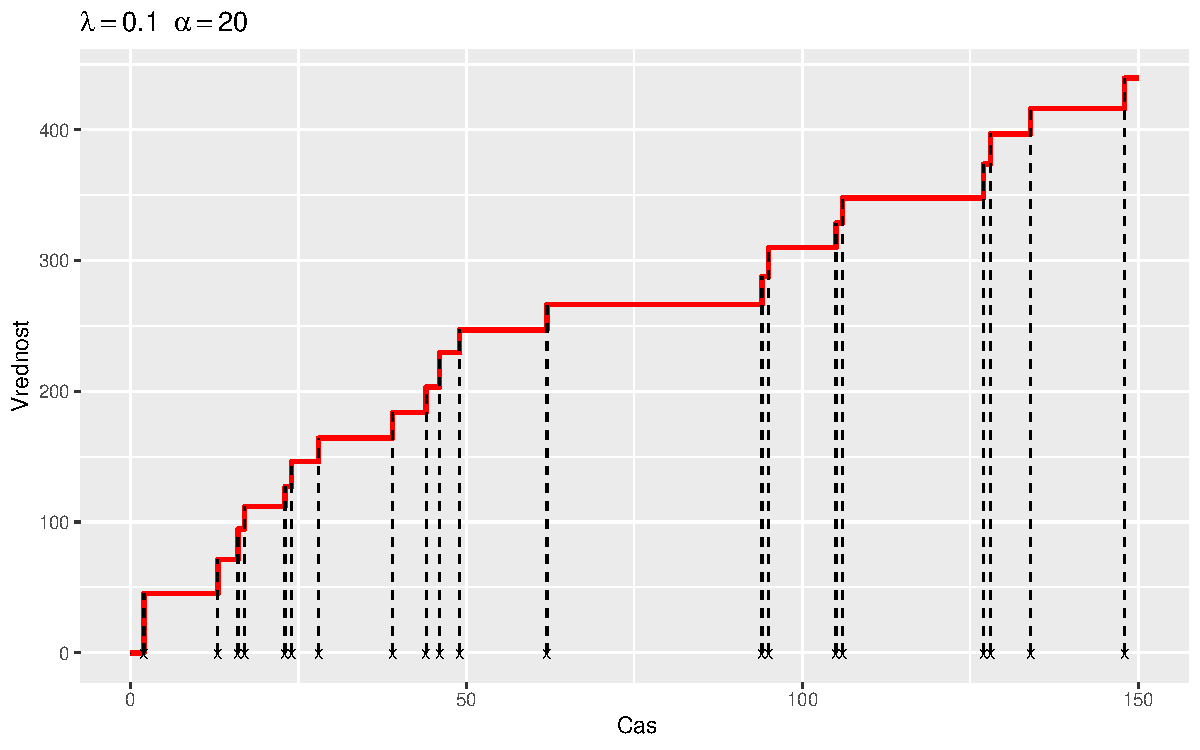
\includegraphics[width=\textwidth]{
            C:/Users/38651/OneDrive - Univerza v Ljubljani/Desktop/Diploma/Diplomski-seminar/GraphsAndPhotos/slika1.pdf
            }
        \caption{Primer trajektorije sestavljenega Poissonovega procesa}
        \label{fig:slika1}
    \end{figure}
    
    \noindent


    \begin{definicija}
        Naj bo $(\Omega, \mathcal{F}, \mathbb{P})$ verjetnostni prostor in naj bo $T\neq\emptyset$
        neprazna indeksna množica ter $(E, \Sigma)$ merljiv prostor. \textit{Slučajni proces}, 
        parametriziran s $T$, je družina slučajnih elementov $X_t : \Omega \to E$,
         ki so $(\mathcal{F}, \Sigma)$-merljivi za vsak $t \in T$.
        \label{def:slucProc}
    \end{definicija}

    \begin{opomba}
        V delu se bomo omejili na primer, ko $T$ predstavlja "cas, torej $T = [0, \infty)$ in da slu"cajne
        spremenljivke 
        zavzemajo vrednosti v realnih "stevilih, torej $(E, \Sigma) = (\R, \B_{\R})$, kjer $\B_\R$ 
        predstavlja Borelovo $\sigma-$algebro na $\R$.
        \label{op:Konvencije}
    \end{opomba}


    \begin{definicija}
        Za fiksen $\omega \in \Omega$ je preslikava 
        $[0, \infty) \rightarrow \mathbb{R}; \ t \mapsto X_t(\omega)$ 
        \textit{trajektorija} oziroma \textit{realizacija} slučajnega procesa $(X_t)_{t\geq0}$.
        Tako lahko slu"cajni proces gledamo kot predpis, ki vsakemu elementu vzor"cnega prostora 
        $\Omega$ priredi slu"cajno funkcijo
        $(X_t(\omega))_{t\geq0}: [0, \infty) \rightarrow \mathbb{R}$.
        \label{def:realizac}
    \end{definicija}

    \begin{definicija}
        Naj bo $(X_t)_{t\geq0}$ slu"cajni proces. Potem za $s < t$ definiramo
        \textit{prirastek procesa} $X_t - X_s$ na intervalu $[s, t]$. Proces $(X_t)_{t\geq0}$ ima 
        \textit{neodvisne prirastke}, če so za vsak nabor realnih "stevil
        $0 \leq t_1 < t_2 < \ldots < t_n < \infty$ prirastki
        $$
            X_{t_2} - X_{t_1}, \ X_{t_3} - X_{t_2}, \ \ldots, \ X_{t_n} - X_{t_{n-1}}
        $$
        med seboj neodvisni.
        \label{def:prirastek}
    \end{definicija}

    \begin{trditev}
        Naj bo $(X_t)_{t\geq0}$ slu"cajni proces na $(\Omega, \F, \mathbb{P})$. Potem ima $(X_t)_{t\geq0}$
        neodvisne prirastke natanko tedaj, ko je za vsak nabor realnih "stevil 
        $0 \leq t_1 < \ldots < t_n < t_{n+1} <\infty$ prirastek $X_{t_{n+1}} - X_{t_n}$ neodvisen od
        slu"cajnega vektorja $(X_{t_1}, \dots, X_{t_n})$.
        \label{trd:ekvivKarakterizacija}
    \end{trditev}

    \begin{proof}
        $(\Rightarrow):$

        $(\Leftarrow):$
    \end{proof}

    \begin{definicija}
        Naj bo $(X_t)_{t\geq0}$ slu"cajni proces. Potem pravimo, da ima proces
        \textit{stacionarne prirastke}, "ce za vsak $s < t$ in vsak $h > 0$ velja, 
        da ima $X_{t+h} - X_{s+h}$ enako porazdelitev kot $X_t - X_s$.
        \label{def:stacPrir}
    \end{definicija}

    \begin{definicija}
        Naj bo $\lambda > 0$. Slučajnemu procesu $(N_t)_{t\geq 0}$, definiranem na verjetnostnem 
        prostoru $(\Omega, \mathcal{F}, \mathbb{P})$ in z vrednostmi v $\N_0$, pravimo 
        \textit{Poissonov proces} z intenzivnostjo $\lambda$, če zadošča naslednjim pogojem:
        \begin{enumerate}
            \item $N_0 = 0$ \ $\Prob$-skoraj gotovo.
            \item $(N_t)_{t\geq 0}$ ima neodvisne in stacionarne prirastke,
            \item Za $0 \leq s < t$ velja $ N_t - N_s \sim\Pois{\lambda(t - s)}$,
        \end{enumerate}
        \label{def:HPP}
    \end{definicija}
\textcolor{red}{
    \begin{opomba}
        Vidimo, da v definiciji ne zahtevamo, da so skoki procesa le +1. To sledi iz...
        \label{op:skoki}
    \end{opomba}
}

\section{Sestavljeni Poissonov proces}

    \begin{center}
        \framebox[\linewidth]{%
    \rule{0pt}{50pt}%
        Povzetek poglavja/krajsi uvod%
        }
    \end{center}
    \begin{definicija}
        Naj bo $(N_t)_{t\geq0}$ Poissonov proces z intenzivnostjo $\lambda$. 
        Naj bo $(X_i)_{i\geq1}$ zaporedje neodvisnih (med sabo in $(N_t)_{t\geq0}$) in enako 
        porazdeljenih slučajnih spremenljivk z vrednostmi v $\mathbb{R}$. Potem je 
        \textit{sestavljeni Poissonov proces} $(S_t)_{t\geq0}$ definiran kot
        $$
            S_t = \sum_{i=1}^{N_t} X_i.
        $$
        \label{def:CPP}
    \end{definicija}

    \begin{opomba}
        Vidimo, da je sestavljeni Poissonov proces posplo"sitev homogenega Poissonovega procesa, saj "ce za
        $X_i$ vzamemo konstantno funkcijo $X_i = 1$ za vsak $i$, dobimo ravno $HPP$. Bolj v splo"snem, "ce za $X_i$ 
        postavimo $X_i = \alpha$, potem velja $S_t = \alpha N_t$.
        \label{op:CPPHPPPovezava}
    \end{opomba}

    V nadaljevanju bomo homogen Poissonov proces z intenzivnostjo $\lambda >0$ ozna"cevali s $HPP(\lambda)$ 
    ali naborom slu"cajnih spremenljivk $(N_t)_{t\geq0}$ (angl. Homogeneous Poisson Process), 
    sestavljeni Poissonov proces pa s $CPP$ ali naborom slu"cajnih spremenljivk $(S_t)_{t\geq0}$ 
    (angl. Compound Poisson Process), kjer bo vsota sledila $HPP(\lambda)$.

    \subsection{Osnovne lastnosti}

        \begin{trditev}
            $CPP$ ima neodvisne in stacionarne prirastke.
            \label{trd:neodvPrirCPP}
        \end{trditev}

        \begin{proof}
            Za nabor realnih "stevil $0 \leq t_1 < t_2 < \ldots < t_n < \infty$ lahko slu"cajne
            spremeljivke $S_{t_i} - S_{t_{i-1}}$ zapi"semo kot
            \begin{align*}
                S_{t_i} - S_{t_{i-1}} &= \sum_{j=N_{t_{i-1}}+1}^{N_{t_i}} X_j. 
            \end{align*}
            Neodvisnost prirastkov sledi po neodvisnosti $X_i$ od $X_j$ za $i\neq j$ in $N_t$. 
            Naj bo $h > 0$ in $s < t$. Potem velja
            \begin{align*}
                S_{t+h} - S_{s+h} &= \sum_{j=N_{s+h}+1}^{N_{t+h}} X_j \\
            \end{align*}
            Vsota ima $N_{t+h} - N_{s+h}$ členov. Ker za $HPP$ velja 
            $N_{t+h} - N_{s+h} \sim N_t - N_s$, je 
            \begin{align*}
                \sum_{j=N_{s+h}+1}^{N_{t+h}} X_j = \sum_{j=N_{s}+1}^{N_{t}} X_j = S_t - S_s.
            \end{align*}
        \end{proof}

        \begin{trditev}
            Naj bo $(S_t)_{t\geq 0}$ $CPP$ in naj bosta $\mu = \E\left[X_i\right] < \infty$ 
            pri"cakovana vrednost in $\sigma^2= \Var{X_i} <\infty$ varianca
            slu"cajnih spremenljivk $X_i$ za vsak $i$. Potem sta za $t\geq0$ pri"cakovana vrednost in 
            varianca $S_t$ enaki 
            \begin{equation*}
                \E\left[S_t\right] = \mu\lambda t \qquad \text{in} \qquad \Var{S_t} = \lambda t\left(\sigma^2 + \mu^2\right).
            \end{equation*}
            \label{trd:PricVarCPP}
        \end{trditev}

        \begin{proof}

            Definiramo slu"cajno spremenljivko
            \begin{equation}
                Y_k = X_1 + X_2 + \cdots + X_k
                \label{eq:Y_k}
            \end{equation}
            in vidimo, da je za $t\geq0$ $S_t$ pogojno na $N_t = k$ enako porazdeljena 
            kot $Y_k$. Tako dobimo 
            \begin{align*}
            \E\left[S_t\mid N_t = k\right] = \E\left[Y_k\right] = k\mu \qquad \text{in} \qquad
            \Var{S_t\mid N_t = k} = \Var{Y_k} = k\sigma^2.
            \end{align*}
            Po formuli za popolno pri"cakovano vrednost velja 
            $\E\left[S_t\right] = \E\left[\E\left[S_t\mid N_t\right]\right]$. Torej

            \begin{align*}
                \E\left[S_t\right] = \E\left[\E\left[S_t\mid N_t\right]\right] = \E\left[\mu N_t\right] = \mu\lambda t.
            \end{align*}

            \noindent
            Prek formule $\Var{S_t} = \E\left[\Var{S_t\mid N_t}\right] + \Var{\E\left[S_t\mid N_t\right]}$ ra"cunamo 

            \begin{equation*}
                \E\left[\Var{S_t\mid N_t}\right] = \E\left[\Var{X_i}N_t\right] = \sigma^2\lambda t
            \end{equation*}
            in 
            \begin{equation*}
                \Var{\E\left[S_t\mid N_t\right]} = \Var{\E\left[X_i\right]N_t} = \mu^2\lambda t,
            \end{equation*}
            saj $N_t\sim\Pois{\lambda t}$. Skupaj dobimo $\Var{S_t} = \lambda t\left(\sigma^2 + \mu^2\right)$.
        \end{proof}

    \subsection{Rodovne funkcije}

    \begin{trditev}
        Naj bo $(S_t)_{t\geq0}$ $CPP$. Naj bodo slu"cajne spremenljivke $X_i$, ki jih se"stevamo v 
        $CPP$ enako porazdeljene kot $X$. Potem ima za $t\geq0$ karakteristi"cna funkcija $\varphi_{S_t}$ 
        obliko
        \begin{equation*}
            \varphi_{S_t}(u) = e^{\lambda t\left(\varphi_X(u) - 1\right)}, 
        \end{equation*}
        kjer $\varphi_X$ ozna"cuje karakteristi"cno funkcijo $X$.
        \label{trd:MomentGener}
    \end{trditev}
    
    \begin{proof}
        \begin{align}
            \varphi_{S_t}(u) 
                    &= \E\left[\exp\left[iuS_t\right]\right] = \nonumber
                        \E\left[\exp\left[iu\sum_{i = 1}^{N_t}X_i\right]\right] \nonumber\\
                    &= \sum_{k=0}^{\infty}
                        \E\left[\exp\left[iu\sum_{i = 1}^{N_t}X_i\mid N_t=k\right]\right]\Prob\left(N_t = k\right) \nonumber \\ 
                    &= \sum_{k=0}^{\infty}
                        \E\left[\exp\left[iu\sum_{i = 1}^kX_i\right]\right]\Prob\left(N_t = k\right) \nonumber \\
                    &= \sum_{k=0}^{\infty}
                        \underbrace{\E\left[e^{iuX}\right]^k}_{\varphi_X(u)^k}\frac{(\lambda t)^k}{k!}e^{-\lambda t} \label{eq:MomentS_t}\\ 
                    &= e^{-\lambda t} + e^{-\lambda t}\sum_{k=1}^\infty\frac{\left(\varphi_X(u)\lambda t\right)^k}{k!} \nonumber \\
                    &= e^{\lambda t\left(\varphi_X(u) - 1\right)} \nonumber
        \end{align}
    \end{proof}

    Hitro lahko vidimo, da sta karakteristi"cna in rodovna funkcija $CPP$ enaki

    \begin{equation*}
        \varphi_{S_t}(u) = e^{\lambda t\left(\varphi_X(u) - 1\right)} \qquad \text{in} \qquad 
        G_{S_t}(u) = e^{\lambda t\left(G_X(u) - 1\right)},
    \end{equation*} 

    \noindent
    saj v splo"snem velja, da je karakteristi"cna funkcija neke slu"cajne spremenljivke $Y$ enaka
    njeni momentno rodovni funkciji izvrednoteni v $iu$, torej $\varphi_Y(u) = G_Y(iu)$. Rodovna pa 
    izverdnotena v $\ln(u)$, torej $G_Y(u) = M_Y(\ln(u))$, "ce obstajata.
    V nadaljevanju bomo uporabljali predvsem karakteristi"cno funkcijo $CPP$, saj je ta vedno definirana 
    za vsak $u\in\R$. Prav nam bo pri"sla tudi naslednja povezava med karakteristi"cno funkcijo $CPP$ 
    in rodovno funkcijo $HPP(\lambda)$.
    \begin{trditev}
        Naj bosta $(S_t)_{t\geq0}$ $CPP$ in $(N_t)_{t\geq0}$ $HPP(\lambda)$ neodvisna. 
        Naj bodo slu"cajne spremenljivke $X_i$, ki jih se"stevamo v $CPP$ enako porazdeljene kot $X$. 
        Potem za fiksen $t\geq0$ velja

        \begin{align*}
            \varphi_{S_t}(u) = G_{N_t}\left(\varphi_{X}(u)\right).
        \end{align*}

        \label{trd:povezavaRodovneKarkateristicne}
    \end{trditev}

    \begin{proof}
        Po ena"cbi (\ref{eq:MomentS_t}) iz trditve \ref{trd:MomentGener} velja, da je $\varphi_{S_t}(u)$ enaka
        \begin{align*}
            \varphi_{S_t}(u) &= \sum_{k=0}^{\infty}
            \varphi_X(u)^n\frac{(\lambda t)^k}{k!}e^{-\lambda t} \\
            &= G_{N_t}\left(\varphi_X(u)\right).
        \end{align*}
    \end{proof}

    \subsection{Porazdelitev CPP}
    Sedaj se posvetimo vpra"sanju, kako je porazdeljena slu"cajna spremenljivka $S_t$ za $t\geq 0$? 
    Iz definicije $HPP(\lambda)$ vemo, da je $N_t$ za $t\geq0$ porazdeljena kot Poissonova slu"cajna 
    spremenljivka s parametrom $\lambda t$. Fiksiramo $t\geq0$ in dobimo 

    \begin{align*}
        F_{S_t}(x) = \Prob(S_t \leq x) 
        &= \sum_{k=0}^\infty \Prob(S_t \leq x \mid N_t = k)\Prob(N_t = k) \\
        & = \sum_{k=0}^\infty \Prob(\sum_{i=1}^k X_i \leq x)\frac{(\lambda t)^k}{k!}e^{-\lambda t} \\
        & = \sum_{k=0}^\infty F_X^{*k}(x)\frac{(\lambda t)^k}{k!}e^{-\lambda t}, \\
    \end{align*}

    \noindent
    kjer je $F_X^{*k}(x)$ porazdelitev $k$-te konvolucije slu"cajne spremenljivke $X$. Razen za 
    posebne primere, je zgornji izraz za prakti"cne namene ne-izra"cunljiv in nam ne pomaga veliko.
    
    \begin{zgled}
        "Ce pogledamo primer, ko so $X_1, X_2, \dots$ neodvisne enako porazdeljene slu"cajne spremenljivke,
        porazdeljene kot $X$
        \begin{equation*}
            X\sim\text{Gamma}(a) \qquad \qquad f_X(x) = \frac{1}{\Gamma(a)}x^{a-1}e^{-x}
        \end{equation*}
        s parametrom $a>0$, lahko pridemo do razmeroma eksplicitne porazdelitve $CPP$. Gostota $k$-te 
        konvolucije $X_1 + \cdots + X_k$ ima formulo
        \begin{equation*}
            f_{X_1 + \cdots + X_k}(x) = \frac{1}{\Gamma(na)}x^{na-1}e^{-x}.
        \end{equation*}
        Za $t\geq 0$ in $x \geq 0$ torej velja
        \begin{align*}
            F_{S_t}(x) = \Prob(S_t \leq x)
            &= \sum_{k=0}^\infty F_X^{*k}(x)\frac{(\lambda t)^k}{k!}e^{-\lambda t}\\
            &= \sum_{k=0}^\infty 
            ...
        \end{align*}

        

    \end{zgled}
    
    %Poka"zimo, da je $CPP$ v resnici porazdeljen, kot limita linearne 
    %kombinacije neodvisnih Poissonovih slu"cajnih spremenljivk. 
    
    \begin{trditev}
        Naj bo $N\sim \Pois{\lambda}$  za $\lambda >0$ in $X_1, X_2, \dots X_n$ neodvisne s.s. (neodvisne 
        med sabo in od $N$) enako porazdeljene kot
        $$ X\sim
        \begin{pmatrix}
            a_1 & a_2 & a_3  \dots & \\
            \tfrac{\lambda_1}{\lambda} & \tfrac{\lambda_2}{\lambda} & \tfrac{\lambda_3}{\lambda} \dots & 
        \end{pmatrix},
        $$
        za poljubne $a_1, a_2, \dots, a_n \in \R$ in 
        $\lambda_1, \lambda_2, \dots, \lambda_n \in \R^+$ za katere velja 
        ${\sum_{i=1}^n\lambda_i = \lambda}$.
        Potem velja 
        \begin{equation*}
            \sum_{j=1}^\infty a_jY_j \sim \sum_{j=1}^NX_j,
        \end{equation*}
        kjer so $Y_1,Y_2,  \dots$ neodvisne s.s.\ porazdeljene kot 
        $\Pois{\lambda_1},\Pois{\lambda_2}, \dots$
        \label{trd:NXjeEnakoaY}
    \end{trditev}

    \begin{proof}
        S $\varphi_{Z_n}(u)$ ozna"cimo karakteristi"cno funkcijo s.s.\ 
        $Z_n := a_1Y_1 + a_2Y_2 + \dots + a_nY_n$ in s $\varphi_{Z}(u)$ karakteristi"cno funkcijo s.s.\
        $Z:= \sum_{j=1}^{N}X_j$. Po neodvisnosti velja
        \begin{align*}
            \varphi_{Z_n}(u) 
                    &= \prod_{j=1}^{n}\varphi_{Y_j}(a_ju)\\
                    &= \prod_{j=1}^{n}\exp\left[\lambda_j\left(e^{a_j i u} - 1\right)\right] \\
                    &= \exp\left[\sum_{j=1}^{n}\lambda_j\left(e^{a_j i u} - 1\right)\right].
        \end{align*}

        \noindent
        Po trditvi \ref{trd:povezavaRodovneKarkateristicne} velja
        \begin{align*}
            \varphi_{Z}(u) 
                    &= G_N\left(\varphi_X(u)\right) \\
                    &= \exp\left[\lambda\left(\varphi_X(u) - 1\right)\right] \\
                    & = \exp\left[\lambda\left(\sum_{j=1}^\infty\frac{\lambda_j}{\lambda}e^{a_jiu} - 1\right)\right]\\
                    &= \exp\left[\sum_{j=1}^{\infty}\lambda_j\left(e^{a_j i u} - 1\right)\right]
        \end{align*}

        \noindent 
        Vidimo, da velja%Rezultat je posledica inverzne formule za karateristi"cne funkcije.
        \begin{equation*}
            \varphi_{Z_n} \xrightarrow{n\to\infty}\varphi_Z,
        \end{equation*}
        torej po Lévijevem izreku o kontinuiteti velja $Z_\infty :=\lim_{n\to\infty}Z_n \sim Z$.
    \end{proof}

    \begin{posledica}
        Naj bo $(a_n)_{n\in\N}$ poljubno zaporedje realnih "stevil in $(\lambda_n)_{n\in\N}$ zaporedje 
        pozitivnih realnih "stevil, za katere velja $\sum_{n=1}^\infty\lambda_n = \lambda$ in 
        \begin{equation*}
            X\sim
            \begin{pmatrix}
                a_1 & a_2 &  \dots \\
                \tfrac{\lambda_1}{\lambda} & \tfrac{\lambda_2}{\lambda} & \dots
            \end{pmatrix}.
        \end{equation*}
        Potem velja
        \begin{equation*}
            \sum_{j=1}^{n}a_jY_j \xrightarrow[n\to\infty]{d}\sum_{j=1}^NX_j,
        \end{equation*}
        \label{pos:NXjeEnakoaYstevno}
    \end{posledica}

    \begin{proof}
        Ker velja $\varphi_{Z_n}(u) \xrightarrow{n\to\infty} \varphi_{Z}(u)$ za vsak $u\in\R$, po Lévijevem
        izreku o zveznosti sledi, da $Z_n \xrightarrow[n\to\infty]{d} Z$.
    \end{proof}

    Kaj pa v primeru, ko so $X_i$ zvezno porazdeljene? 
    Tedaj se problema lotimo na slede"c na"cin. Definiramo $F_n(x) := F(\tfrac{m}{n})$ kjer je
    $F(x)$ porazdelitvena funkcija slu"cajne spremenljivke $Z_n$ in 
    $m = \min\{k \in \mathbb{Z} \mid \tfrac{k}{n} > F_n(x)\}$.

        \begin{figure}[H]
            \begin{center}
            
                \begin{tikzpicture}
                    % coordinate system
                    \draw[->] (-0.75,0) -- (9,0) node[right] {$x$};
                    \draw[->] (2,0) -- (2,4.5) node[above] {$F, F_n$};
                    \draw (2, 3.4) -- (2, 3.4) node[left] {$1$};
                    \draw[dashed] (-0.75,3.2) -- (9,3.2);
                
                    % CDF of continuous random variable
                    \draw[blue] (-0.75, 0.1) .. controls (0,0.2) and (2.2, 0.3) .. (2.8, 1.2);
                    \draw[->, blue] (2.8, 1.2) .. controls (3.1, 1.7) and (3.6, 2) .. (5, 2.1);
                    \filldraw[blue] (5, 2.5) circle (0.7pt);
                    \draw[blue] (5, 2.5) .. controls (6, 2.8) and (7.5, 3) .. (9, 3.15) node[below] {$F(x)$};
                
                    % CDF of F_n, 
                    \draw[->, red] (-0.75, 0.22) -- (0.25, 0.22);
                    \filldraw[red] (-0.75, 0.22) circle (0.7pt);
                    \draw[->, red] (0.25, 0.39) -- (1.25, 0.39);
                    \filldraw[red] (0.25, 0.39) circle (0.7pt);
                    \draw[->, red] (1.25, 0.74) -- (2.25, 0.74);
                    \filldraw[red] (1.25, 0.74) circle (0.7pt);
                    \draw[->, red] (2.25, 1.68) -- (3.25, 1.68);
                    \filldraw[red] (2.25, 1.68) circle (0.7pt);
                    \draw[->, red] (3.25, 2.01) -- (4.25, 2.01) node[above left]{$F_n(x)$};
                    \filldraw[red] (3.25, 2.01) circle (0.7pt);
                    \draw[->, red] (4.25, 2.58) -- (5.25, 2.58);
                    \filldraw[red] (4.25, 2.58) circle (0.7pt);
                    \draw[->, red] (5.25, 2.79) -- (6.25, 2.79);
                    \filldraw[red] (5.25, 2.79) circle (0.7pt);
                    \draw[->, red] (6.25, 2.94) -- (7.25, 2.94);
                    \filldraw[red] (6.25, 2.94) circle (0.7pt);
                    \draw[->, red] (7.25, 3.07) -- (8.25, 3.07);
                    \filldraw[red] (7.25, 3.07) circle (0.7pt);
                
                
                    %intervals of F_n
                
                \end{tikzpicture}
                \caption{Aproksimacija $F$ s $F_n$}
                \label{fig:slika2}
            \end{center}
        \end{figure}

    \noindent
    Kot je razvidno iz slike \ref{fig:slika2}, je $F_n(x)$ stopni"casta funkcija, ki aproksimira 
    porazdelitveno funkcijo $F(x)$. Velja $F_n \xrightarrow{n\to\infty}F$ povsod kjer je $F$ zvezna.



    %\noindent
    %"Ce sedaj po"sljemo $n \to \infty$, dobimo
    %\begin{align}
    %    \varphi_{Z}(u) := \lim_{n\to\infty}\varphi_{Z_n}(u) = e^{\sum_{j=1}^{\infty}\lambda_j\left(e^{a_j i u} - 1\right)}.
    %    \label{eq:karFunkcVrste}
    %\end{align}
%
    %\noindent
    %Kot smo izpeljali zgoraj je karakteristi"cna funkcija $CPP$ podana s predpisom
%
    %\begin{align*}
    %    \varphi_{S_t}(u) = e^{\lambda t\left(\varphi_X(u) - 1\right)}, 
    %\end{align*}
%
    %\noindent
    %kar lahko zapi"semo kot 
%
    %\begin{align*}
    %    \varphi_{S_t}(u) = e^{\lambda t\int_{\R}\left(e^{i u z} - 1\right) \mu(dz)},
    %\end{align*}
%
    %\noindent
    %kjer je $\mu := X*\Prob$ potisk mere naprej po s.s.\ $X$. Prav tako lahko (\ref{eq:karFunkcVrste}) zapi"semo
    %kot 
%
    %\begin{align*}
    %    \varphi_{Z}(u) = e^{\int_{\R}\left(e^{i u x} - 1\right)\nu(dx)},
    %\end{align*}
%
    %\noindent
    %Za neko ustrezno mero $\nu$. Vidimo, da ko po"sljemo $n\to \infty$, za ustrezen izbor 
    %$a_1, a_2, \dots$ in $\lambda_1, \lambda_2, \dots$ karakteristi"cna funkcija 
    %vrste $Z_n$ konvergira h karakteristi"cni funkciji $S_t$. Torej po Lévijevem izreku o zveznosti 
    %sledi, da je $S_t$ enako porazdeljena kot $Z = \sum_{i=1}^{\infty}\alpha_iY_i$.
%

    \subsection{CPP kot martingal}

        \begin{definicija}
            Slu"cajni proces $X_t$ prilagojen glede na filtracijo $(\F_t)_{t\geq0}$
            martingal, "ce velja 
            $$
                \E\left[X_t\mid\F_s\right] = X_s
            $$
            za vsak $0\leq s \leq t$.
            \label{def:martingal}
        \end{definicija}

        Poka"zimo, da v splo"snem $CPP$ ni martingal.

        \begin{trditev}
            Naj bo $(S_t)_{t\geq0}$ $CPP$ z intenzivnostjo $\lambda>0$ in naj bodo $X_i$ neodvisne
            in enako porazdeljene slu"cajne spremenljivke z $\E\left[X_i\right] = \mu$ za vsak $i$.
            Potem je $S_t$ martingal natanko tedaj, ko je $\mu = 0$.
            \label{trd:CPPnimartingal}
        \end{trditev}

        \begin{proof}
            Naj bo $0\leq s\leq t$. Potem velja
            \begin{align*}
                \E\left[S_t\mid\F_s\right] 
                        &= \E\left[S_t - S_s + S_s\mid \F_s\right] \\
                        &= \E\left[S_t - S_s\right] + \E\left[S_s\mid \F_s\right] \\
                        &= \mu\lambda(t-s) + S_s
            \end{align*}
           Enakost $\mu\lambda(t-s) + S_s = S_s$ velja $\iff$ $\mu\lambda(t-s) = 0 \iff \mu = 0$.
        \end{proof}

        \begin{opomba}
            Seveda, "ce velja $\mu \geq 0$, potem je $S_t$ submartingal, "ce pa $\mu \leq 0$, je
            $S_t$ supermartingal.
        \end{opomba}

        \begin{trditev}
            Naj bo $(S_t)_{t\geq0}$ CPP z intenzivnostjo $\lambda > 0$ in naj bodo $X_i$ neodvisne
            in enako porazdeljene slu"cajne spremenljivke z $\E\left[X_i\right] = \mu$ za vsak $i$,
            Potem je proces 
            $$
                S_t - \mu\lambda t
            $$
            martingal.
            \label{trd:CPPpostanemartingal}
        \end{trditev}

        \begin{proof}
            Naj bosta $0 \leq s < t$. Prirastek $S_t - S_s$ je neodvisen od $\F_s$ in ima 
            pri"cakovano vrednost $\mu\lambda(t-s)$. Torej 
            \begin{align*}
                \E\left[S_t - \mu\lambda t\mid\F_s\right] 
                        &= \E\left[S_t - S_s\right] + S_s - \mu\lambda t\\
                        &= \mu\lambda(t-s) + S_s - \mu\lambda t\\
                        &= S_s - \mu\lambda s.
            \end{align*}
        \end{proof}

        %\subsection{"Cas prvega prehoda}
        %Postavimo si vpra"sanje, kdaj bo $CPP$ prvi"c dosegel nek $a\in\R$. Obravnavajmo primer, ko je 
        %$a>0$, saj je primer, ko je $a$ negativen simetri"cen. Naj bo $T_a = \inf\{t\geq0; S_t \geq a\}$ 
        %"cas prvega prehoda $CPP$. V tem poglavju bomo izra"cunali porazdelitev $T_a$.
        %"Ce pogledamo dogodek $\{T_a \leq t\}$.

\section{Cramér-Lundbergov model}

    \begin{center}
        \framebox[\linewidth]{%
    \rule{0pt}{50pt}%
        zgodovinski uvod in uporaba%
    }
    \end{center}

    \subsection{Proces tveganja in verjetnost propada}
        \begin{definicija}
            Naj bo $(S_t)_{t\geq0 }$ $CPP$.\textit{Proces tveganja} v Cramér-Lundbergovem modelu definiramo kot
            \begin{align*}
                U_t = u + p(t) - S_t,
            \end{align*}
            kjer je $u \geq 0$ za"cetni kapital zavarovalnice in $p(t)$ funkcija prihodkov iz premij. 
            \label{def:procesTveganja}
        \end{definicija}

        \begin{opomba}
            Vrednost $U_t$ predstavlja kapital zavarovalnice ob "casu $t\geq0$. Standardno je za $p(t)$ 
            vzeti deterministi"cno (celo linearno) funkcijo $p(t) = ct$, kjer je $c$ stopnja prihodkov premij.
            \label{op:procesTveganja}
        \end{opomba}

        Propad bomo definirali kot dogodek, ko bo vrednost procesa tveganja postala negativna.

        \begin{definicija}
            \textit{Propad} definiramo kot dogodek, da proces tveganja $(U_t)_{t\geq0}$ kadarkoli pade pod $0$. 
            Torej 
            \begin{align*}
                \bigl\{U_t<0 \ \text{za} \ t\geq 0\bigr\}
            \end{align*}
            in "casu
            \begin{align*}
                T = \inf\{t\geq0 \mid U_t < 0\}, 
            \end{align*}
            pravimo \textit{"cas propada}. Seveda velja enakost med dogodkoma
            \begin{align*}
                \{U_t<0 \ \text{za} \ t\geq0\} = \{T<\infty\}.
            \end{align*}
            \label{def:PropadCasPropada} 
        \end{definicija}

        \begin{definicija}
            \textit{Verjetnost propada} je definirana kot funckija $\psi(u): (0,\infty) \to [0,1]$ 
            podana s predpisom
            \begin{align*}
                \psi(u) = \Prob(T<\infty \mid U_0 = u).
            \end{align*}
            \label{def:VerjetnostPropada}
        \end{definicija}

        \begin{definicija}
            Po konstrukciji procesa tveganja $(U_t)_{t\geq0}$ je verjentost propada mogo"ca le ob 
            prihodih, ki sledijo $HPP(\lambda).$ S $T_n$ ozna"cimo "cas $n$-tega prihoda in definiramo 
            \textit{ogrodje} procesa tveganja kot $(U_{T_n})_{n\in\N}$.
            \label{def:ogrodjeProcesaTveganja}
        \end{definicija}

         S pomo"cjo ogrodja procesa tveganja lahko dogodek propada zapi"semo kot
        \begin{align*}
            \biggl\{\inf_{t\geq0}U_t<0\biggr\} &= \biggl\{\inf_{n\in\N}U_{T_n}<0\biggr\} \\
                          &= \biggl\{\inf_{n\in\N}\left(u + p(T_n) - S_{T_n}\right) < 0\biggr\} \\
                          &= \biggl\{\inf_{n\in\N}\left(u + cT_n - \sum_{i=1}^nX_i\right) < 0\biggr\} \\
        \end{align*}
        in tako dobimo nov na"cin kako zapisati verjetnost propada. Za $n\in\N$ z $W_n$ ozna"cimo 
        medprihodni "cas $HPP(\lambda)$, torej $W_n := T_n - T_{n-1}$ in $W_0 = T_0 = 0$. Definiramo 
        izgubo $n$-tega prihoda kot 
        \begin{equation*}
            Y_n := X_n - cW_n \quad \text{za} \ n\in\N.
        \end{equation*}
        Ozna"cimo z $Z_n := \sum_{i=1}^nY_i$ in dobimo
        \begin{equation*}
            \psi(u) = \Prob\left(\sup_{n\in\N}\left(Z_n\right) > u\right).
        \end{equation*}
        Tako verjetnost propada prevedemo na prehodno verjetnost diskretnega slu"cajnega 
        sprehoda $(Z_n)_{n\in\N}$. V nadaljevanju nas bo predvsem zanimalo asimptoti"cno 
        vedenje $\psi(u)$, ko gre $u\rightarrow\infty$. Cilj obravnavanja verjetnosti propada v 
        Cramér-Lundbergovem modelu je, da se izognemo 
        propadu z verjetnostjo 1 oziroma, da je verjetnost, da $(Z_n)_{n\in\N}$ prese"ze $u$
        tako majhna, da lahko v praksi dogodek propada izklju"cimo. V nadaljevanju bomo
        predpostavili, da sta $\E\left[X_n\right]$ in $\E\left[W_n\right]$ kon"cni. To nam 
        zagotovi, da je $\E\left[Z_n\right] = \sum_{i=1}^n\E\left[X_i\right] - c\E\left[W_i\right]$
        kon"cna.

        Ker pa velja ena od treh mo"znosti:
        \begin{align*}
            \E\left[Y_n\right] = 
            \begin{cases}
                > 0, & \text{za} \ c\E\left[W_n\right] > \E\left[X_n\right], \\
                = 0, & \text{za} \ c\E\left[W_n\right] = \E\left[X_n\right], \\
                < 0, & \text{za} \ c\E\left[W_n\right] < \E\left[X_n\right],
            \end{cases}
        \end{align*}
        bo $\E\left[Z_n\right]$ divergirala bodisi proti $\infty$ bodisi proti $-\infty$ in celo v 
        primeru $\E\left[Y_n\right] = 0$ bo verjetnost propada enaka 1, ker bosta obstajali 
        pozdaporedji $(n_k)_{k\in\N}$ in $(m_k)_{k\in\N}$... Spitzer [138] je dokazano.

        \begin{definicija}
            Pravimo, da proces tveganja $(U_t)_{t\geq0}$ izpolnjuje \textit{pogoju neto zaslu"zka}
            (ang. \textit{net profit condition}), "ce velja 
            \begin{equation*}
                c > \frac{\E\left[X\right]}{\E\left[W\right]}.
            \end{equation*}
            Pogoj bomo v nadaljenvanju imenovali NPC.
            \label{def:NPC}
        \end{definicija}
    
    \subsection{Lundbergova neenakost/lahko repne porazdelitve/small claim case/ cramer bound}

        V poglavju se bomo ukvarjali z lahkorepnimi porazdelitvami.
        \begin{definicija}
            Pravimo, da ima slu"cajna spremenljivka $X$ \textit{lahkorepno porazdelitev}, "ce velja
        \begin{equation*}
            \E\left[e^{uX}\right] = M_X(u) < \infty \quad \text{za} \ u \in (-\varepsilon, \varepsilon)
        \end{equation*}
        za nek $\varepsilon > 0$.
        \label{def:lahkorepnaPorazdelitev}
        \end{definicija}

        \begin{definicija}
            Naj za slu"cajn spremenljivko $Z_1$ obstaja njena momentno--rodovna funkcija 
            na intervalu $u\in(-\varepsilon, \varepsilon)$  za nek $\varepsilon > 0$. "Ce obstaja 
            enoli"cna re"sitev ena"cbe
            \begin{equation*}
                M_{Z_1}(l)  = 1,
            \end{equation*}
            pravimo $l$ \textit{Lundbergov koeficient}.
        \end{definicija}


    \subsection{Simulacija majhnih zahtevkov}


    \subsection{tezkorepne porazdelitve/large claim case}


    \subsection{Simulacija velikih zahtevkov}


        



        
        

























\section*{Slovar strokovnih izrazov}

%\geslo{}{}
%
%\geslo{}{}
%


% seznam uporabljene literature
\begin{thebibliography}{99}

\bibitem{1}S.E. Shreve, Stochastic Calculus for Finance II: Continuous-Time Models, Springer, (2004).
\bibitem{2}S.M. Ross, Stochatic Processes: Second Edition, Wiley, (1996).
\bibitem{3}P. Embrechts, C. Klüppelberg, T. Mikosch, Modelling Extremal Events: For Insurance and Finance, Springer, (1997).
\bibitem{4}T.Mikosch, Non-Life Insurance Mathematics: An Introduction with the Poisson Process, Springer, Second Edition, (2009).
\end{thebibliography}

\end{document}